
\documentclass[9pt]{beamer-control}
\usepackage{beamer-control-prac}
\begin{document}

\TOPIC[1]{System Response}
\CONCEPT[1]{Week 1: Introduction to software and hardware}

\begin{frame}
\frametitle{Introduction}
In this practical, you will learn how to interface with the real-time hardware in the CARM Laboratory using Matlab/Simulink.

\vfill

This practical will consist of the following parts:
\begin{itemize}
\item Setting up
\item Operating the hardware
\item Filtering the output
\end{itemize}
\end{frame}

\SUBCONCEPT{Setting up}

\begin{frame}{Hardware}
Get into a small group, and acquire 
\begin{itemize}
	\item a QUBE unit,
	\item a green printed circuit board (PCB),
	\item a power cable,
	\item and a red inertia disk.
\end{itemize}  

These components only assemble one way. In particular, ensure the ribbon cable is inserted correctly into the PCB (align the notch on the ribbon cable connector with the corresponding gap in the plastic PCB connector).

\textcolor{red}{Insert image of components}


\end{frame}


\begin{frame}{Software}
Once the physical plant is assembled, 
\begin{enumerate}
\item Download the Simulink model QubeModel.slx from Canvas
\item Open this file in Matlab 2026b/Simulink and save it in a separate folder named “Week\_1”
\item Create a Matlab script named “Week\_1” to accompany your Simulink file
\end{enumerate}

Saving your weekly progress will be essential in this course in order to draw upon in later weeks. Note that no spaces or special characters are permitted in Matlab file or path names.

\end{frame}



\SUBCONCEPT{Operating the hardware}

\begin{frame}{Inputs and outputs}
The block in the Simulink model contains the code needed to interface with the QUBE. For the purposes of these practicals we have simplified the inputs and outputs. 

\begin{itemize}
	\item \textbf{Input} - voltage that eventuates as a torque on the attached disk, in volts
	\item \textbf{Output} - angle from the initial position, in radians
\end{itemize}

\textcolor{red}{Figure of QUBE in Simulink}


\end{frame}




\begin{frame}{Operating the QUBE}
	Now that the input and outputs are understood, we may begin operating and controlling the device
	\begin{enumerate}
		\item For an initial input, insert a step function block (Step) with default parameters (Hint: click anywhere and type “step”), this will generate a step signal, i.e. a 0 volts for 1 second, and 1 volt after 1 second
		\item Also attach a Scope block to the output of the plant to read the angular displacement
		\item You may then build the model (ctrl-B) and connect to the target and then run (note that building the model may take up to 60 seconds)
	\end{enumerate}

\end{frame}

\begin{frame}{Operating the QUBE}
	The following figure labels the important functions on the toolbar under the Hardware tab and shows the simple Simulink model.
\begin{figure}
	\centering
	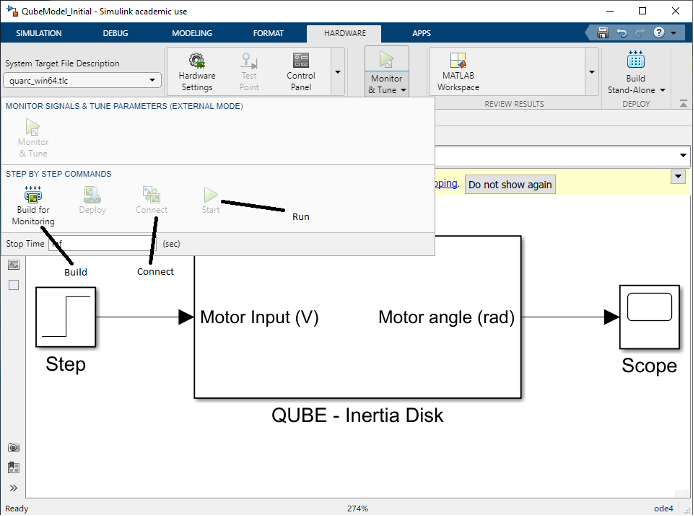
\includegraphics[width=8cm]{prac1_simulink.png}
	\caption{Simulink toolbar.}
\end{figure}
\end{frame}


\begin{frame}{Calibration}
	The output angle is measured using an encoder which divides the range of motion into discrete ``ticks” which approximate the current position. In this case, the range of positions (1 revolution) is divided into 2048 ticks. Therefore, the encoder output (in ticks) may be converted to radians by multiplying by $\tfrac{2\pi}{2048}$ (this is done within the Simulink QUBE subsystem). In general it is critical to understand the format of the output from the device for control purposes i.e. units, scale, resolution, sensitivity etc. 
\end{frame}

\begin{frame}{Discretisation}
	The following figure demonstrates the discretisation of the encoder.
	\begin{figure}
		\centering
		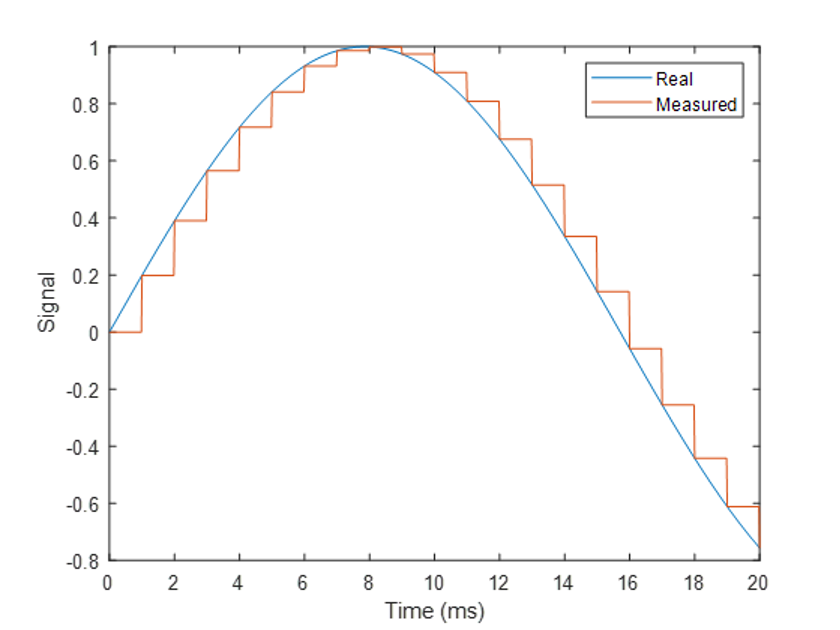
\includegraphics[width=8cm]{prac1_discretised_signal.png}
		\caption{Discretised signal from encoder.}
	\end{figure}
	
\end{frame}


\SUBCONCEPT{Filtering the output}

\begin{frame}{Low-pass filter}
Sensors will always contain measurement noise, and digital sensors will be discretised. In future, when we wish to feedback our signal for control purposes, we must filter the signal to attenuate this noise (typically high frequencies) and remove the effects of discretisation. For this we will use a low pass filter using the block called Transfer Fcn. 

The low pass filter has transfer function
\[
G(s) = \frac{f_c}{s+f_c},
\]
and may be constructed by selecting a cut off frequency in radians per second ($f_c$), after which the signal is attenuated.

\end{frame}


\begin{frame}{Low-pass filter}
The discrete steps from the encoder can be effectively smoothed out by the low pass filter by removing the higher frequencies required to form the sharp edge. 
\begin{enumerate}
	\item Add the low-pass filter Transfer Fcn block to the output signal
	\item Connect a scope before and after the filter to visualise the effects of filtering
	\item Run the QUBE and compare the pre-filtered and filtered signals to get an intuitive feel for an appropriate cut off frequency
\end{enumerate}

 A good guess might be 50 rad/s to start, but experiment with different cutoff frequencies to get an idea of what range we need. The key is to get a smooth signal without introducing too much time lag. 
\end{frame}

\begin{frame}{Low-pass filter}
\textcolor{red}{Change figure to one you would get from open loop inertia disk}
The following figure shows that the filter does smooth the curve, but also introduces a time lag (i.e. shifts to the right).
\begin{figure}
	\centering
	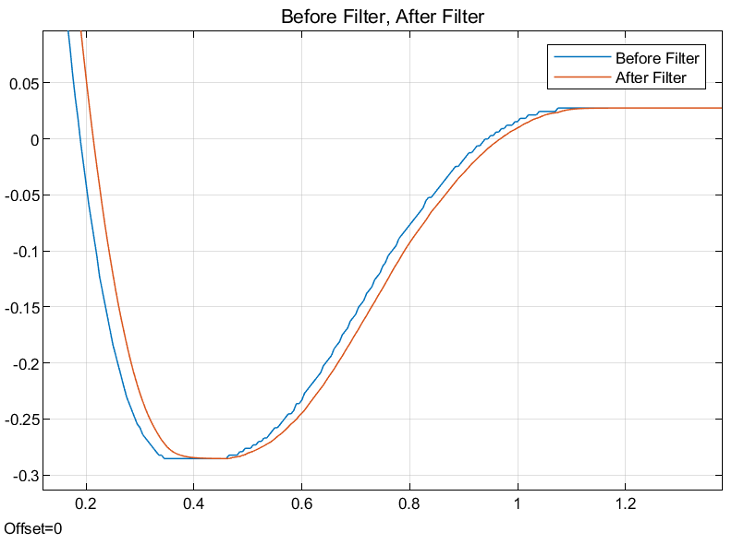
\includegraphics[width=8cm]{prac1_filter.png}
	\caption{Output signal before and after filter.}
\end{figure}
\end{frame}

\begin{frame}{Next week}
	This week you learned how to set up and operate the QUBE, and filter the output signal.
	
	For control purposes, it is often very beneficial to first derive a model or characterise the output response of a system. Next week we will step through these processes for the QUBE inertia disk system.
\end{frame}

\end{document}
